\chapter{Spezifikationen}

\section{Use Cases} \label{sec:UseCases}
\begin{figure}[ht!]
    \centering
    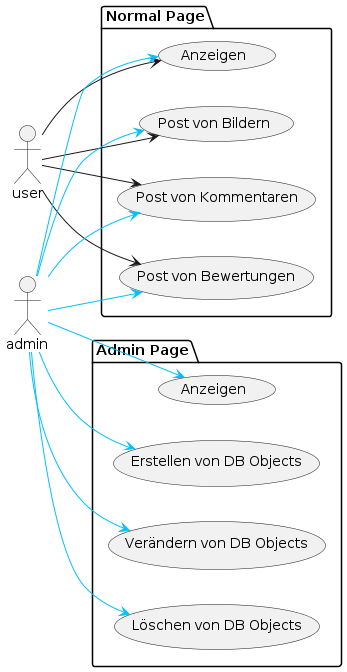
\includegraphics[width=0.45\textwidth]{images/Use Case.png}
    \caption{Use Cases}
    \label{fig:UseCases}
\end{figure}

Die Use Cases für den User sind nur auf der eigentlichen WebApp, während Admins
neben der WebApp noch Zugriff auf ein Admin Panel haben. Das Admin Panel ist
eine Web Page der WebApp, wo Admins direkt auf die Datenbank zugreiffen können.



\newpage

\section{Anforderungen} \label{sec:Anforderungen}
\subsection{Menus} \label{spez:Menus}

Dateien:
\begin{itemize}
    \item core/views.py (\ref{code:core.views.py})
    \item core/models.py (\ref{code:core.models.py})
    \item core/statistic\_functions.py (\ref{code:core.statistic-functions.py})
\end{itemize}

Menus sind Objekte, welche in der Datenbank als \code{Menu}-Objekt gespeichert
werden (siehe \ref{fig:DB}, \ref{code:core.models.py}). Jedes \code{Menu} ist
ein Vorkommen eines Gerichts. Um die verschiedenen Vorkommen der
\code{Menu}-Objekte zu gruppieren existiert das \code{MenuType}-Objekt.
Menus mit dem selben Namen wird der gleiche \code{MenuType} zugeordnet. 

Die Menus werden von der offiziellen Mensa Webseite gescraped. Die
Synchronization (siehe \ref{spez:Webscraper}) findet bei jedem Aufruf einer der
Seiten statt.

Nur wenn das heutige Datum mit dem Datum des Menus übereinstimmt, ist es
möglich, Bilder zu posten (siehe \ref{spez:Images}), das Menu zu bewerten (siehe
\ref{spez:Rating}) und die Posts zu liken (siehe \ref{spez:Liking}).

\subsection{Webscraper} \label{spez:Webscraper}
 
Dateien:
\begin{itemize}
    \item core/webscraper.py (\ref{code:core.webscraper.py})
    \item core/models.py (\ref{code:core.models.py})
\end{itemize}

Der Webscraper ist ein standalone Python Script (siehe
\ref{code:core.webscraper.py}), womit die Menu-Daten der MensaRating WebApp und
die Daten der Offiziellen Webseite synchronisiert werden. 

Der Webscraper stellt mit der Library \code{requests} Anfragen an die Webseite
\url{https://neuekanti.sv-restaurant.ch/de/menuplan/}. Dabei werden die Tages-
und Datumsdaten von der Seite geladen und danach werden die Gerichte (Name,
Beschreibung, Vegan/Vegetarisch) gescraped.

Das Script wird bei jedem Aufruf der Webseite ausgeführt. Nach dem Scraping der
Daten werden diese mit der Datenbank (siehe \ref{fig:DB}) verglichen. Für jedes
Menu auf der offiziellen Webseite wird überprüft, ob es an dem Tag bereits ein
\code{Menu}-Objekt (siehe \ref{spez:Menus}) mit dem selben Namen in der
Datenbank gibt. Wenn nicht, dann wird ein neues \code{Menu}-Objekt erstellt. Dem
neuen \code{Menu}-Objekt wird der zugehörige Menutype, welcher den Namen mit dem
Menu gemeinsam hat, zugeordnet. Existiert dieser Menutype noch nicht, so wird
auch dieser in der Datenbank erstellt. (siehe \ref{code:core.models.py})

Existiert in der Datenbank bereits ein anderes Menu als auf der offiziellen
Webseite, so wird das alte Menu gelöscht. Dadurch kann die MensaRating WebApp
Änderungen auf der offiziellen Webseite entdecken und übernehmen.

\begin{lstlisting}
    data = scrape_data()
    for index, menu, date in data:
        menus = get_menus_from_db(date=date)
            if menu[index] exists:
                menu_type = get_menu_type(menu=menu)
                if menu_type == null:
                    menu_type = create_menu_type(menu, data)
                update_menu(menu[index], data)
            else:
                menu_type = get_menu_type(menu=menu)
                if menu_type == null:
                    menu_type = create_menu_type(menu, data)
                create_menu(data, menu_type)
    
    // Cleanup
    all_menu_types = get_all_menu_types()
    for i in all_menu_types:
        if len(get_menus_from_db(menu_type=i)) == 0:
            delete_menu_type(i)
\end{lstlisting}

(Code in \code{core/webscraper.py})

\subsection{Bilder Gallerie} \label{spez:Gallerie}

Dateien:
\begin{itemize}
    \item static/js/imageSlideshow.js
    \item core/statistic\_functions.py (\ref{code:core.statistic-functions.py})
\end{itemize}

Die Bildergallerie ist ein Frontend Feature und wurde mit dem Tutorial von
folgender Seite erstellt:
\url{https://www.w3schools.com/howto/howto_js_slideshow.asp}. Die Bildergallerie
wird gebraucht, damit die Images (siehe \ref{spez:Images}) der Menus (siehe
\ref{spez:Menus}) angezeigt werden können.

Im Javascript werden die verschiedenen Bilder in einem Array gespeichert. Nur
das aktive Bild bekommt den style \code{display: block}. Die anderen Bilder
haben \code{display: none}. Wenn es noch keine Bilder von einem Menu gibt, dann
wird ein default Bild angezeigt.

Da Bilder im  sein können, werden sie mit ihren Dimensionen
auf ihre Orientierung überprüft. Wenn das Bild Hochformat ist, dann wird es im
css anders behandelt.

Bilder werden ihrer Orientierung (Hoch- oder Querformat) entsprechend im Design
der Webseite anders eingebunden. Die Orientierung eines Bildes wird mit dem
folgenden Code Ausschnitt determiniert:

\begin{lstlisting}
for (let index = 0; index < images.length; index++) {
      const element = images[index];
      if (element.naturalHeight > element.naturalWidth && !element.className.includes("portrait")) {
          // The image is a portrait and needs to be resized
          element.style.objectFit = "contain";
      }
  }
\end{lstlisting}

Die Reihenfolge der Bilder ist absteigend nach der Anzahl \emph{Likes} (siehe
\ref{spez:Liking}) Likes, die jedes Bild hat, sortiert


\subsection{Posts} \label{spez:Posts}

Dateien:
\begin{itemize}
    \item core/forms.py 
    \item core/post\_functions.py
    \item core/models.py (\ref{code:core.models.py})
    \item core/views.py (\ref{code:core.views.py})
\end{itemize}

Der Begriff ``Posts'' beschreibt zwei verschiedene Objekte in der Datenbank (siehe
\ref{fig:DB}). Es gibt kein übergeordnetes Post-Objekt. Als Posts werden Images
(siehe \ref{spez:Images}) und Reviews (siehe \ref{spez:Reviews}) bezeichnet.

Ein Post (siehe \ref{spez:Rating}) ist nur möglich, wenn das zugehörige
\code{Menu} vom selben Tag ist. Posts können auch nur am selben Tag geliked
werden (siehe \ref{spez:Liking}).

Um einen Post zu veröffentlichen, schickt der User ein \code{POST-HTML-Form} (siehe code/forms.py) an
das Backend durch die \code{menu} funktion in \code{core/views.py}
\ref{code:core.views.py}. Es wird bestimmt, ob der Post ein \code{Image} oder
ein \code{Review} ist und dem entsprechend in \code{post\_function.py}
ausgewertet. Durch eine Rückmeldung in Form einer \code{Pop-Up Message} wird der
User über den Erfolg oder Misserfolg seines Posts informiert.

\subsubsection{Images} \label{spez:Images}

Es gibt ein \code{Image}-Objekt in der Datenbank (siehe \ref{fig:DB}). Die Image
Datei wird nicht in der Datenbank gespeichert. Stattdessen wird die Referenz auf
die Image Datei gespeichert

Wenn das Image auf der öffentlichen Webseite (siehe \ref{spez:Deployment})
angezeigt wird, dann wird das Image nicht auf dem eigentlichen Server
gespeichert, sondern auf einem Google Drive. Das wird gemacht, da der Server
keine Möglichkeit hat, Daten anhaltend speichern zu können.

\subsubsection{Reviews} \label{spez:Reviews}

Es gibt ein \code{Review}-Objekt in der Datenbank (siehe \ref{fig:DB}). Ein
Review ist ein Kommentar zu einem Menu (\ref{spez:Menus}), welcher auf der
Webseite angezeigt wird.

\subsubsection{Liking} \label{spez:Liking} Dateien
\begin{itemize}
    \item static/js/app.js
    \item core/views.py (\ref{code:core.views.py})
\end{itemize}

Posts kann man liken. Dabei wird das \code{Like} Attribut des zugehörigen Posts
in der Datenbank (siehe \ref{fig:DB}) erhöht. Um zu verhindern, dass ein User
einen Post mehrfach liken kann, werden die Likes des Users im Javascript
Localstorage gespeichert. Die Likes haben kein eigenes Objekt in der Datenbank,
weil dadurch zu viele Einträge entstehen würden.

Das Like Verfahren ist in Javascript in \code{static/js/app.js} programmiert.
Von da aus wird die Aktion des Users an das Backend (siehe \code{like} in
core/views.py \ref{code:core.views.py}) geschickt und dort in der Datenbank
gespeichert.

\subsection{Rating} \label{spez:Rating}

Dateien:
\begin{itemize}
    \item core/models.py (\ref{code:core.models.py})
    \item core/statistic-functions.py (\ref{code:core.statistic-functions.py})
    \item core/views.py (\ref{code:core.views.py})
\end{itemize}

Ein \code{Rating} ist ein Objekt in der Datenbank (siehe \ref{fig:DB}) und stellt
eine Bewertung für ein \code{Menu}-Objekt (siehe \ref{spez:Menus}) dar. Ein
Rating hat einen Wert zwischen 1 und 5 und kann nur gegeben werden, wenn das
zugehörige Menu vom selben Tag ist.

Von den Ratings eines Menus wird in \code{core/statistic-functions.py}
\ref{code:core.statistic-functions.py} der Durchschnitt berechnet, um diesen auf
der Webseite anzuzeigen


\subsection{Statistik: Filter und Sortierung} \label{spez:Statistik}

Dateien:
\begin{itemize}
    \item core/views.py (\ref{code:core.views.py})
    \item core/statistic\_functions.py (\ref{code:core.statistic-functions.py})
    \item static/js/allmenu\_statistics.js (\ref{code:static.js.allmenu-statistics.js})
\end{itemize}

Auflistungen von Menus können gefiltert und sortiert werden. Folgende Filter
können durch einen Button ausgewählt werden: nur vegan, nur vegetarisch und kein
Filter. Folgende Sortierungen können durch einen Button ausgewählt werden:
Rating-Durchschnitt (absteigend), Alphabetisch, Anzahl Ratings (absteigend) und Anzahl
Vorkommen (absteigend und nur unter der Seite `alle Menus', weil nur \code{MenuType}
Objekte diese Attribut besitzen).

Beim Neuladen der Seite werden die Daten aller Menus in der Auflistung aus der
Datenbank gesammelt (bei der Seite `alle Menus' (siehe \ref{code:core.views.py})
werden alle \code{MenuType}-Objekte anstelle der Menus angezeigt) und
standardmässig nach dem Rating-Durchschnitt sortiert. 

Das Filtern und Sortieren auf Knopfdruck erfolgt in Javascript. Die einzelnen
\code{<div>} Elemente im HTML Code, die ein Element der Auflistung beschreiben,
sind standardmässig leer und werden durch die Javascript Funktion
\code{updateListboxs()} in \code{static/js/allmenu\_statistics.js}
(\ref{code:static.js.allmenu-statistics.js}) mit den Daten der Menus oder
MenuTypes gefüllt. Diese Daten sind pro Menu in einem Javascript Object
gespeichert:

\begin{lstlisting}
    menuType = {
        url: data.url,
        name: data.name,
        index: data.index,
        rating: data.rating,
        occurrences: data.occ,
        numrates: data.numrates,
        vegan: data.vegan,
        vegetarian: data.vegetarian,
        visible: true
    }
\end{lstlisting}

(Code in \code{core/templates/allMenu.html})

Je nach Filter wird das visible Attribut auf \code{false} gesetzt, wodurch die
Daten des zugehörigen Menus oder MenuTypes in der Auflistung nicht mehr
angezeigt werden (In CSS: \code{display: none}). Das passiert ebenfalls durch
die \code{updateListboxs()} Funktion.

\newpage

\subsection{Account System} \label{spez:Account}

Dateien:
\begin{itemize}
    \item users/models.py (\ref{code:users.models.py})
    \item users/views.py (\ref{code:users.views.py})
\end{itemize}

Die Entwicklung des Account Systems ist stark von folgendem Django Tutorial
inspiriert:
(\url{https://www.youtube.com/playlist?list=PL-osiE80TeTtoQCKZ03TU5fNfx2UY6U4p}).
Allerdings wurde der Code in verschiedenen Projekten bereits verwendet und
unterscheidet sich mittlerweile stark vom Tutorial

Django hat ein eingebautes Account System. Dieses Account System wird in die
Webseite integriert (siehe \ref{code:users.views.py}). Es bietet folgende
Funktionen:
\begin{itemize}
    \item register
    \item login
    \item logout
    \item password-reset
    \item password-reset-done
    \item password-reset-confirm
    \item password-reset-complete
\end{itemize}

Beim Registrieren wird ein \code{User}-Objekt in der Datenbank (noch nicht in
der models.py Datei) erstellt. Danach wird ein \code{Profil}-Objekt (siehe
\ref{code:users.models.py} und \ref{fig:DB}) erstellt. Beim Registrieren gibt es
ausserdem eine ReCaptcha-Überprüfung (siehe \ref{code:users.views.py}), damit
die Datenbank nicht von Spam durch Bots überfallen wird. Eine Email-Verifikation
gibt es nicht.

Die Login und Logout funktionen sind direkt von Django implementiert (siehe users/urls.py)

Die Funktion des Password Reset funktioniert über die angegebene Email Adresse.
Es wird ein sicherer Token für den Password Reset an die Email Adresse gesendet.
Die Email wird über einen Gmail Account versendet.


\subsection{Punktesystem (Karma)} \label{spez:Karma}

Dateien:
\begin{itemize}
    \item core/models.py (\ref{code:core.models.py})
    \item core/statistic\_functions.py (\ref{code:core.statistic-functions.py})
\end{itemize}

Die Erfahrungspunkte, auch Karma genannt, werden als Attribut in
\code{Profil}-Objekten (siehe \ref{fig:DB}) gespeichert. User erhalten Punkte
für das Veröffentlichen von Posts (siehe \ref{spez:Posts}) und für Likes auf
eigenen Posts. (Funktion \code{add\_karma\_for\_posting}). Mit den Punkten kann
ein User Achievements erreichen (siehe \ref{spez:Badges}).

\subsection{Achievements (Badges)} \label{spez:Badges}

Dateien:
\begin{itemize}
    \item core/models.py (\ref{code:core.models.py})
    \item core/statistic\_functions.py (\ref{code:core.statistic-functions.py})
\end{itemize}

Die Achievements werden als \code{Badge}-Objekt in der Datenbank (siehe
\ref{fig:DB}) gespeichert. Die Objekte werden keinem User zugeordnet.
Stattdessen wird immer, wenn die Achievements eines Users angezeigt werden
sollen, berechnet, welche Achievements dieser User hat. Daher sind die Objekte
in der Datenbank nur eine Beschreibung, welche Achievements es gibt.

\begin{lstlisting}
    def get_badges_of_profil(profil):
        badges = Badge.objects.all()
 
        img_counter = count_best_image_of_profil(profil=profil)
        review_counter = count_best_review_of_profil(profil=profil)
        karma = profil.karma

        categories = [karma, img_counter, review_counter]

        highest_badge = [null, null, null]
        for i in badges:
            if i.count <= categories[i.condition_category]:  # Does the profil own the badge?
                if highest_badge[i.condition_category] is null:
                    highest_badge[i.condition_category] = i
                else:
                    if highest_badge[i.condition_category].count < i.count:
                        highest_badge[i.condition_category] = i
        
        highest_badges = [i for i in highest_badges if i is not None]  # Remove null badges
\end{lstlisting}

(Code in \code{core/statistic-functions.py})

Es gibt 3 verschiedene Kategorien von Achievements.
\begin{itemize}
    \item Karma-basiert (siehe \ref{spez:Karma})
    \item Images-basiert (siehe \ref{spez:Images})
    \item Review-basiert (siehe \ref{spez:Reviews})
\end{itemize}

Karma-basiert heisst, dass der User ein Achievment erhält, wenn er eine
bestimmte Menge an Karma hat. Image- und Review-basiert heisst, dass der User
eine bestimmte Anzahl an `most liked Images/Reviews' in einem MenuType (siehe
\ref{spez:Menus}) braucht, um das Achievement zu erhalten.

Erhält der User ein neues Achievements in einer Kategorie so wird das letzte
Achievement durch das neue ersetzt. Der User kann Achievements auch wieder
verlieren, wenn er die Kriterien dafür nicht mehr erfüllt.

Alle erreichten Achievements werden auf der Profil Seite angezeigt (siehe
\ref{code:core.views.py}).



\subsection{Deployment}\label{spez:Deployment}

Dateien:
\begin{itemize}
    \item Procfile
    \item requirements.txt
    \item .github/workflows/CI Tests.yml
\end{itemize}

Die Webseite wird auf einem Heroku Eco Dyno gehostet. Die Datenbank wird ebenfalls
von Heroku auf einem Postgres Server gehostet. Die Bilder werden auf einer
Google Drive gespeichert (siehe \ref{spez:Images}).

Dieses Projekt wird mit Heroku deployed, weil Heroku eine einfache \code{Django}
Deployment Plattform ist und viele Anleitung im Internet dazu verfügbar sind.
Heroku beitet ausserdem viele Addons, welche für Weiterentwicklungen und
Veröffentlichungen nützlich sein können.
